%% ----------------------------------------------------------------
%% Thesis.tex -- MAIN FILE (the one that you compile with LaTeX)
%% ---------------------------------------------------------------- 

% Set up the document
\documentclass[a4paper, 11pt, oneside]{Thesis}  % Use the "Thesis" style, based on the ECS Thesis style by Steve Gunn
\graphicspath{Figures/}  % Location of the graphics files (set up for graphics to be in PDF format)

% Include any extra LaTeX packages required
\usepackage[square, numbers, comma, sort&compress]{natbib}  % Use the "Natbib" style for the references in the Bibliography
\usepackage{verbatim}  % Needed for the "comment" environment to make LaTeX comments
\usepackage{vector}  % Allows "\bvec{}" and "\buvec{}" for "blackboard" style bold vectors in maths
\hypersetup{urlcolor=blue, colorlinks=false}  % Colours hyperlinks in blue, but this can be distracting if there are many links.

%% ----------------------------------------------------------------
\begin{document}
\frontmatter      % Begin Roman style (i, ii, iii, iv...) page numbering

% Set up the Title Page
\title  {Optimal Team Formation in Fantasy Basketball}
\authors  {{Anthony Mazzawi}}
\addresses  {\groupname\\\deptname\\\univname}  % Do not change this here, instead these must be set in the "Thesis.cls" file, please look through it instead
\date       {September 2017}
\subject    {}
\keywords   {}

\maketitle
%% ----------------------------------------------------------------

\setstretch{1.3}  % It is better to have smaller font and larger line spacing than the other way round

% Define the page headers using the FancyHdr package and set up for one-sided printing
\fancyhead{}  % Clears all page headers and footers
\rhead{\thepage}  % Sets the right side header to show the page number
\lhead{}  % Clears the left side page header

\pagestyle{fancy}  % Finally, use the "fancy" page style to implement the FancyHdr headers

%% ----------------------------------------------------------------
% Declaration Page required for the Thesis, your institution may give you a different text to place here
\Declaration{

\addtocontents{toc}{\vspace{1em}}  % Add a gap in the Contents, for aesthetics

I, Anthony Mazzawi, declare that this thesis titled, `Optimal Team Formation in Fantasy Basketball' and the work presented in it are my own. I confirm that:

\begin{itemize} 
\item[\tiny{$\blacksquare$}] This work was done wholly or mainly while in candidature for a research degree at this University.
 
\item[\tiny{$\blacksquare$}] Where any part of this thesis has previously been submitted for a degree or any other qualification at this University or any other institution, this has been clearly stated.
 
\item[\tiny{$\blacksquare$}] Where I have consulted the published work of others, this is always clearly attributed.
 
\item[\tiny{$\blacksquare$}] Where I have quoted from the work of others, the source is always given. With the exception of such quotations, this thesis is entirely my own work.
 
\item[\tiny{$\blacksquare$}] I have acknowledged all main sources of help.
 
\item[\tiny{$\blacksquare$}] Where the thesis is based on work done by myself jointly with others, I have made clear exactly what was done by others and what I have contributed myself.
\\
\end{itemize}
 
 
Signed:\\
\rule[1em]{25em}{0.5pt}  % This prints a line for the signature
 
Date:\\
\rule[1em]{25em}{0.5pt}  % This prints a line to write the date
}
\clearpage  % Declaration ended, now start a new page

%% ----------------------------------------------------------------
% The "Funny Quote Page"
%\pagestyle{empty}  % No headers or footers for the following pages

%\null\vfill
% Now comes the "Funny Quote", written in italics
%\textit{``Write a funny quote here.''}

%\begin{flushright}
%If the quote is taken from someone, their name goes here
%\end{flushright}

%\vfill\vfill\vfill\vfill\vfill\vfill\null
%\clearpage  % Funny Quote page ended, start a new page
%% ----------------------------------------------------------------

% The Abstract Page
\addtotoc{Abstract}  % Add the "Abstract" page entry to the Contents
\abstract{
\addtocontents{toc}{\vspace{1em}}  % Add a gap in the Contents, for aesthetics

This will be a dissertation on the optimal team formation in fantasy basketball. 
}

\clearpage  % Abstract ended, start a new page
%% ----------------------------------------------------------------

\setstretch{1.3}  % Reset the line-spacing to 1.3 for body text (if it has changed)

% The Acknowledgements page, for thanking everyone
\acknowledgements{
\addtocontents{toc}{\vspace{1em}}  % Add a gap in the Contents, for aesthetics

I would like to thank my advisor Dr. Ramchurn Sarvapali for his support throughout the entirety of my project.

}
\clearpage  % End of the Acknowledgements
%% ----------------------------------------------------------------

\pagestyle{fancy}  %The page style headers have been "empty" all this time, now use the "fancy" headers as defined before to bring them back


%% ----------------------------------------------------------------
\lhead{\emph{Contents}}  % Set the left side page header to "Contents"
\tableofcontents  % Write out the Table of Contents

%% ----------------------------------------------------------------
\lhead{\emph{List of Figures}}  % Set the left side page header to "List if Figures"
\listoffigures  % Write out the List of Figures

%% ----------------------------------------------------------------
\lhead{\emph{List of Tables}}  % Set the left side page header to "List of Tables"
\listoftables  % Write out the List of Tables

%% ----------------------------------------------------------------
\setstretch{1.5}  % Set the line spacing to 1.5, this makes the following tables easier to read
\clearpage  % Start a new page
\lhead{\emph{Abbreviations}}  % Set the left side page header to "Abbreviations"
\listofsymbols{ll}  % Include a list of Abbreviations (a table of two columns)
{
% \textbf{Acronym} & \textbf{W}hat (it) \textbf{S}tands \textbf{F}or \\
\textbf{NBA} & \textbf{N}ational \textbf{B}asketball \textbf{A}ssociation\\
\textbf{MDP} & \textbf{M}arkov \textbf{D}ecision \textbf{P}rocess\\
}

%% ----------------------------------------------------------------
%\clearpage  % Start a new page
%\lhead{\emph{Physical Constants}}  % Set the left side page header to "Physical Constants"
%\listofconstants{lrcl}  % Include a list of Physical Constants (a four column table)
%{
% Constant Name & Symbol & = & Constant Value (with units) \\
%Speed of Light & $c$ & $=$ & $2.997\ 924\ 58\times10^{8}\ \mbox{ms}^{-\mbox{s}}$ (exact)\\

%}

%% ----------------------------------------------------------------
\clearpage  %Start a new page
\lhead{\chaptername}  % Set the left side page header to "Symbols"
\listofnomenclature{lll}  % Include a list of Symbols (a three column table)
{
% symbol & name & unit \\
$\lambda$ & Poisson Mean \\
$\alpha$ & Offensive Rating \\
$\beta$ & Defensive Rating \\
$\gamma_h$ & Home Court Advantage \\
$\rho$ & Time\\
}
%% ----------------------------------------------------------------
% End of the pre-able, contents and lists of things
% Begin the Dedication page

\setstretch{1.3}  % Return the line spacing back to 1.3

%\pagestyle{empty}  % Page style needs to be empty for this page
%\dedicatory{For/Dedicated to/To my\ldots}

\addtocontents{toc}{\vspace{2em}}  % Add a gap in the Contents, for aesthetics


%% ----------------------------------------------------------------
\mainmatter	  % Begin normal, numeric (1,2,3...) page numbering
\pagestyle{fancy}  % Return the page headers back to the "fancy" style

% Include the chapters of the thesis, as separate files
% Just uncomment the lines as you write the chapters

\chapter{Introduction}

\section{Motivation}

\section{Objectives}

\section{Report Structure}
Chapter 2 will provide the background necessary for the report.  Chapter \ref{chapter:data} provides an insight into the data collected and used for the project.  Chapter \ref{chapter:model} develops a statisical model, based on the English football model of Dixon and Coles \citep{dixon_coles}.  The betting market is analysed in Chapter \ref{chapter:betting}.  Finally, Chater \ref{chapter:conclusion} concludes the paper by offering suggestions for improvements.

\chapter{Literature Review}\label{chapter:background}

\textit{Give a background on basketball, sports predictions in general, sports predictions on basketball and theoretical concepts used in the report.}

\section{Analytics in Sports}


\subsection{Baseball}
Baseball can be seen as the beginning for sports analytics \citep{moneyball}.  The Oakland Athletics could not compete financially with the bigger teams of Major League Baseball, thus general manager Billy Beane used 
\subsection{American Football}

\subsection{English Football}
Dixon and Coles developed a model that uses full-time scores to predict the probabilities of a future match \citep{dixon_coles}.

Dixon and Robinson extended the model created by Dixon and Coles by modelling goal times \citep{dixon_robinson}.

\section{Prediction in the National Basketball Association}
\textit{Talk about the history of data science in the NBA}

\textit{Talk about nba advanced stats.}

% Streak Shooting
There is a belief among basketball players and fans that a player will be more likely to score following a previous successful shot rather than a miss.  A survey was conducted of NBA fans, where 91\% of fans believed that a player has a better chance of scoring after having just made his last two or three shots than after missing the same number \citep{nba_hot_hand}.  Shooting records from the Philadelphia 76ers and it's opponents were analysed from the 1980-81 season.   The analysis provided no evidence towards streak shooting.  Free throw data from the Boston Celtics during the 1980-81 and 1981-82 seasons were also analysed to remove the presence of shot selection and defensive pressure.  Again, no evidence was found the second free throw was affected by the first.  Finally, an experiment with the players from Cornell University as an alternative way to eliminate shot selection and defensive pressure \citep{nba_hot_hand}.  The conclusion of the Cornell experiment is that previous shots 
influenced the players' predictions, but not their performance.  

% Team Cohesion
Team cohesion is an important factor to consider as research studies have shown that highly cohesive teams are likely to be highly successful teams \citep{team_cohesion}.  Research was done to evaluate team cohesion and performance in the basketball league in Kenya \citep{basketball_team_cohesion}.  The participants were athletes who had at least two years experience in the league.  Six players were randomly selected from each team in the league.  The results show that 96\% of players believed they played and won as a team while 76\% believed they lost as a team.  An analysis of variance (ANOVA) test was conducted, which shows that teams with a higher cohesion between players won more frequently than teams with low cohesion.  There was a significant relationship shown between team size and team cohesion.  In the NBA, there is a maximum amount of players allowed per team, so this may not affect this league on the same level.  While the studies show that team cohesion leads to success, it would be difficult to translate that into a statistical model.

% NBA Defense
Most of basketball advanced metrics have been developed for offence as offensive performance is more easily measured due to the number of statistics pertaining to scoring.  Although there are statistics such as steals and blocks that provide some insight into a player's defensive performance, they do not show the full story.  Thus, there have been attempts to model defensive performance by introducing new defensive metrics utilising the the emerging forms of player tracking information \citep{nba_defense}.  The model created by Franks et. al. \citep{nba_defense} begins by estimating defensive matchups for every moment in a basketball game.  The matchups allows us to see which defenders are responsible for which attacking player at different stages of an offensive possession, including when points are scored.  Table \ref{table:defensive_metrics} shows the metrics introduced.  These metrics make it easier to see who are the best and worst defenders in the league and could greatly improve the performance of a statistical model.

\begin{table}[ht]
\centering
\begin{tabular}{|l|l|}
\hline
\textbf{Defensive Metric} & \textbf{Description} \\ \hline
Volume Score & \begin{tabular}[c]{@{}l@{}}The total number of shot attempts a defender faces.\end{tabular}\\ \hline
Disruption Score & \begin{tabular}[c]{@{}l@{}}A defender's ability to reduce the \\  effectiveness of his opponent's shots.\end{tabular}\\ \hline
Defensive Shot Chart & \begin{tabular}[c]{@{}l@{}}Similar to an offensive shot chart, but\\ for defensive shots against.\end{tabular}\\ \hline
Shots Against & \begin{tabular}[c]{@{}l@{}}Weighted average of shots attempted\\ against the defender per 100 possessions.\end{tabular}\\ \hline
Counterpoints & \begin{tabular}[c]{@{}l@{}}Weighted average of points scored\\ against the defender per 100 possessions.\end{tabular}\\ \hline

\end{tabular}
\caption{Defensive Player Metrics}
\label{table:defensive_metrics}
\end{table}

% Shot Selection
Shot selection is a very important part of offence in basketball.  \ldots can capture the correlation between a player's skill and shooting habits.
Shot selection \cite{nba_spatial_analysis}.

% NBA Taxonomy
Again, player tracking data was analysed to dissect basketball plays using acceleration \citep{nba_taxonomy}.  Further research in this subject could lead to classifying team philosophies and using that information when predicting opposing play styles (For example a high tempo offence against a very lax defence)

% Fuzzy Classification
A fuzzy classification system has been developed to predict the winner of a game from the Asociaci\'on de Clubes de Baloncesto, the professional basketball league in Spain \citep{nba_fuzzy_prediction}.  Eight different feature selection algorithms were used and the most consistent features selected were the average number of assists by the first team, the teams' evaluations and the average points scored by each team.  Eleven different fuzzy algorithms were used, with accuracies ranging from 63.5\% to 71.5\%.

\section{Mathematical Concepts}
The following section will describe the mathematical concepts used in the modelling done in this report.

\subsection{Poisson Distribution}
The Poisson distribution is defined by the formula \cite{poisson}

\begin{equation}
p_x(\lambda) = \frac{e^{-\lambda}\lambda^x}{x!}
\end{equation}

Figure \ref{fig:poisson} shows the probability mass function for the Poisson distribution with various $\lambda$.  The $y$ axis is the probability of $k$ occurring given the mean $\lambda$.  \textit{Cite This ->} The function is only defined at integer values of $k$.

\begin{figure}[!htb]
	\centering
	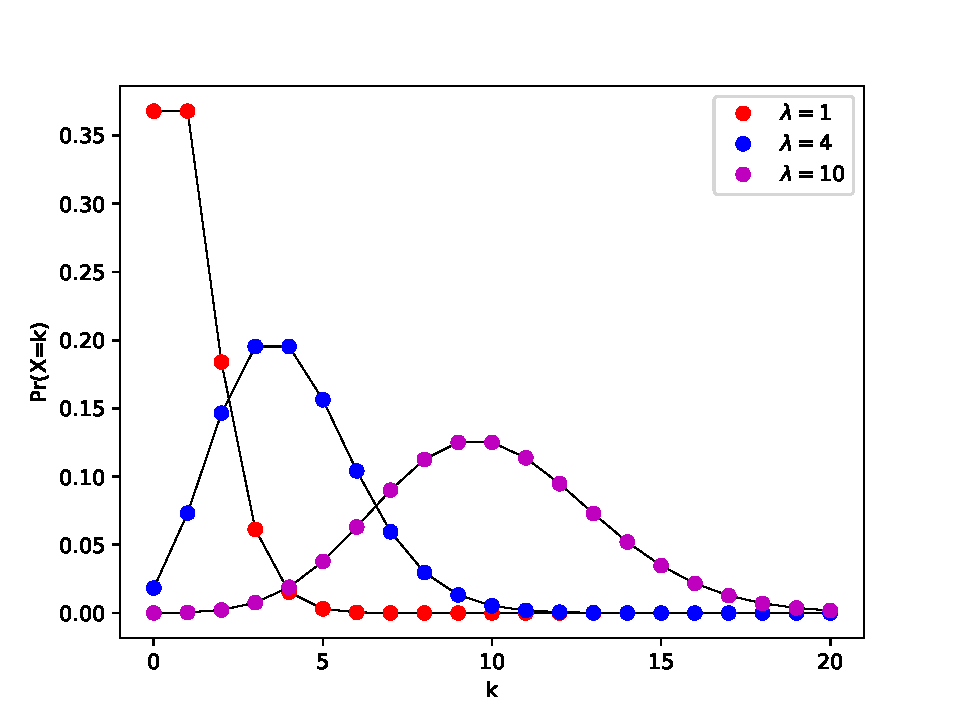
\includegraphics[width=0.75\textwidth]{{Figures/poisson_dist.pdf}}
	\captionof{figure}{Probability mass function of the Poisson Distribution}
	\label{fig:poisson}
\end{figure}

\subsection{Beta Distribution}

The Beta distribution is a probability distribution defined on the interval $[0, 1]$

\chapter{Data}\label{chapter:data}

\textit{Talk about how much data there is, }

The NBA has been shifting towards data analytics in the past few years.  The evolution began in baseball with the book Moneyball.  For this project, the data used will be game logs for players and teams in the past few seasons

\textit{Introduce how there is a lot of NBA data and how the NBA is shifting towards analytics.  Talk about the sources and collection and storage.}

\section{Data Sources}
The data for the National Basketball Association is publicly available on a number of different platforms.  For this project, Basketball-Reference \citep{basketball_reference} was used.  Historical betting odds were also required.  They were obtained from BetExplorer \citep{betting_odds}.  Unfortunately, historical prop betting on basketball was not available anywhere.  Thus, the betting analysis will be limited only to scorelines.

\section{Data Collection}

Using the Beautiful Soup library \cite{beautifulsoup}, the data was scraped.

\section{Betting Odds}

In addition to predicting the winner of a game, betting odds allow another use case for the model.
A description of different betting odds. \cite{betting_odds}

\begin{table}[ht]
\centering
\begin{tabular}{|l|l|}
\hline
\textbf{Bet Type} & \textbf{Description} \\ \hline
Money Line & Bet on the winner of the game. \\ \hline
Spread & Bet on score difference between two teams. \\ \hline
Over/Under & Bet on the total number of points scored \\ \hline
\end{tabular}
\caption{Betting Types}
\label{my-label}
\end{table}


\chapter{Team Model}\label{chapter:team_model}

When evaluating players, it is very important to realize that the team they play for and their opponent will have a strong influence on their performance no matter the skill level.
\textit{Find something that states a player is directly affected by their team}

\section{Dixon and Coles}
Dixon and Coles set out to create a model that incorporates team's attacking and defending abilities \cite{dixon_coles}.

Dixon and Coles created a model with the aim of developing a profitable betting strategy for English football \cite{dixon_coles}.  The model assumes that the amount of goals scored by the home and away sides in any match are independent Poisson variables.  The means are determined by the attack and defence attributes of each side \cite{dixon_coles}.

Dixon and Robinson extended the previously discussed model by using the time each goal was scored instead of only the full time scores \cite{dixon_robinson}. 

\subsection{Model}

There are features 

\begin{itemize}
	\item The model should incorporate the different abilities of both teams.
	\item There should be an advantage for the team playing at home.
	\item The team abilities should be based on a summary of their recent games.
	\item A team's ability is likely to 
	\item When evaluating a team's performance, the ability of the opposing team should be taken into account.
	
\end{itemize}

The base assumption of the model is that the goals scored by the home and away teams are independent Poisson variables.  In a match between teams $i$ and $j$, the number of goals scored by the home and away teams are denoted by

$$X_{ij} ~ \text{Poisson}(\alpha_i\beta_j\gamma_h)$$
$$Y_{ij} ~ \text{Poisson}(\alpha_j\beta_i)$$

where $X_{ij}$ and $Y_{ij}$ are independent, $\alpha_i, \beta_i > 0.$

Dixon and Coles present the following to determine the probabilities of goals scored in a match.

\begin{equation}
\text{Pr}(X_{ij}=x, Y_{ij} = y) = \tau_{\lambda,\mu}(x, y)\frac{\lambda^x\exp(-\lambda)}{x!}\frac{\mu^y\exp(-\mu)}{y!}
\end{equation}

where

$$\lambda = \alpha_i\beta_j\gamma_h$$
$$\mu = \alpha_j\beta_i$$

and

\[
	\tau_{\lambda,\mu}(x,y) = 
	\begin{cases}
		1 - \lambda \mu \rho & \text{if } x=y=0,\\
		1 + \lambda \rho & \text{if } x=0,y=1,\\
		1 + \mu \rho & \text{if } x=1,y=0,\\
		1 - \rho & \text{if } x=1,y=1,\\
		1 & \text{otherwise}.
	\end{cases}
\]	

Dixon and Coles state that .  In the model, $\rho$ is a dependence parameter where $\rho=0$ corresponds to independence.  Basketball and football are fundamentally different sports, thus this dependence parameter is ignored for the basketball model.  

\subsection{Parameter Estimation}

From model \ref{eq:dc_likelihood} with $n$ teams, there are the attack abilities $\{\alpha_1,\ldots,\alpha_n\}$, defence abilities $\{\beta_1,\ldots,\beta_n\}$ and the home advantage parameter $\gamma$ to be estimated.  The constraint

$$\frac{1}{n}\sum_{i=1}^{n}\alpha_i = 1$$

is imposed by Dixon and Coles to keep the model from being over-parameterized.  For the basketball model, this constraint will be equal to 100 due to basketball scores being much higher than football.  

To estimate The National Basketball Association has 30 teams, thus the model has 61 parameters.  With matches indexed $k=1,\ldots,N$, and scores $(x_k, y_k)$, the likelihood function takes the form of



\begin{equation} \label{eq:dc_likelihood}
L(\alpha_i,\beta_i,\gamma, i=1,\ldots,n) = \prod_{k=1}^{N} \exp(-\lambda_k)\lambda_{k}^{x_k}\exp(-\mu_k)\mu_{k}^{y_k}
\end{equation}

where

$$\lambda_k = \alpha_{i(k)}\beta_{j(k)}\gamma,$$
$$\mu_k = \alpha_{j(k)}\beta_{i(k)}$$

The team abilities for the NBA can be seen in Table \ref{table:dc_141516}.  Using these numbers, and selecting the team with the highest probability of winning a game.  The accuracy of selecting a winner was 63.84\% and the value betting strategy won 57.84 units with 37.06\% winning bets.

\begin{table}[t]
	\centering
	\caption{Parameter estimates from the 2014, 2015 and 2016 NBA season using the Dixon Coles model implemented for Basketball}
	\begin{tabular}{|l|c|c|}
		\hline
		\textbf{Team}  & \textbf{$\hat{\alpha}$} & \textbf{$\hat{\beta}$} \\ \hline
		Atlanta Hawks  & 100.902 & 0.985\\ \hline
		Boston Celtics & 99.962 & 1.010\\ \hline
		Brooklyn Nets  & 97.400 & 1.013\\ \hline
		Charlotte Hornets & 96.978 & 0.976\\ \hline
		Chicago Bulls & 97.688 & 0.969\\ \hline
		Cleveland Cavaliers & 101.066 & 0.990\\ \hline
		Dallas Mavericks & 102.960 & 1.008 \\ \hline
		Denver Nuggets & 101.646 & 1.038\\ \hline
		Detroit Pistons & 99.256 & 1.012\\ \hline
		Golden State Warriors & 108.000 & 0.995\\ \hline
		Houston Rockets & 104.750 & 1.017 \\ \hline
		Indiana Pacers & 97.358 & 0.957 \\ \hline
		Los Angeles Clippers & 104.578 & 0.984\\ \hline
		Los Angeles Lakers & 98.553 & 1.052 \\ \hline
		Memphis Grizzlies & 95.980 & 0.947\\ \hline
		Miami Heat & 97.829 & 0.969\\ \hline
		Milwaukee Bucks & 96.464 & 1.006\\ \hline
		Minnesota Timberwolves & 101.166 & 1.038\\ \hline
		New Orleans Pelicans & 99.337 & 1.007\\ \hline
		New York Knicks & 95.207 & 0.996\\ \hline
		Oklahoma City Thunder & 105.347 & 1.000\\ \hline
		Orlando Magic & 97.111 & 1.015\\ \hline
		Philadelphia 76ers & 95.430 & 1.0518\\ \hline
		Phoenix Suns & 101.608 & 1.027\\ \hline
		Portland Trail Blazers & 103.534 & 1.002\\ \hline
		Sacramento Kings & 101.560 & 1.040\\ \hline
		San Antonio Spurs & 102.417 & 0.943\\ \hline
		Toronto Raptors & 101.480 & 0.984 \\ \hline
		Utah Jazz & 94.453 & 0.956\\ \hline
		Washington Wizards & 99.983 & 0.999\\ \hline
		\multicolumn{2}{|c|}{\textbf{Home Court Advantage}} & 1.025\\ \hline
	\end{tabular}
	\label{table:dc_141516}
\end{table}


On October 25th 2016,

\begin{table}[t]
	\centering
	\caption{Parameter estimates from October26th, 2016}
	\begin{tabular}{|l|c|c|}
		\hline
		\textbf{Team}  & \textbf{$\hat{\alpha}$} & \textbf{$\hat{\beta}$} \\ \hline
		Atlanta Hawks  & 100.605 & 0.985\\ \hline
		Boston Celtics & 102.261 & 1.010\\ \hline
		Brooklyn Nets  & 97.253 & 1.013\\ \hline
		Charlotte Hornets & 99.197 & 0.976\\ \hline
		Chicago Bulls & 99.028 & 0.969\\ \hline
		Cleveland Cavaliers & 101.748 & 0.990\\ \hline
		Dallas Mavericks & 100.795 & 1.008 \\ \hline
		Denver Nuggets & 100.306 & 1.038\\ \hline
		Detroit Pistons & 99.567 & 1.012\\ \hline
		Golden State Warriors & 110.88 & 0.995\\ \hline
		Houston Rockets & 104.392 & 1.017 \\ \hline
		Indiana Pacers & 98.837 & 0.957 \\ \hline
		Los Angeles Clippers & 102.403 & 0.984\\ \hline
		Los Angeles Lakers & 95.761 & 1.052 \\ \hline
		Memphis Grizzlies & 96.519 & 0.947\\ \hline
		Miami Heat & 97.311 & 0.966\\ \hline
		Milwaukee Bucks &96.664 & 1.001\\ \hline
		Minnesota Timberwolves & 99.781 & 1.036\\ \hline
		New Orleans Pelicans & 99.503 & 1.020\\ \hline
		New York Knicks & 94.808 & 0.991\\ \hline
		Oklahoma City Thunder & 106.614 & 1.006\\ \hline
		Orlando Magic & 98.861 & 1.018\\ \hline
		Philadelphia 76ers & 94.973 & 1.044\\ \hline
		Phoenix Suns & 99.095 & 1.039\\ \hline
		Portland Trail Blazers & 102.744 & 1.010\\ \hline
		Sacramento Kings & 102.875 & 1.053\\ \hline
		San Antonio Spurs & 101.040 & 0.918\\ \hline
		Toronto Raptors & 100.860 & 0.973 \\ \hline
		Utah Jazz & 94.318 & 0.931\\ \hline
		Washington Wizards & 101.000 & 1.011\\ \hline
		\multicolumn{2}{|c|}{\textbf{Home Court Advantage}} & 1.035\\ \hline
	\end{tabular}
	\label{table:dc_oct2016}
\end{table}


\subsection{Model Limitation and Modification}

The main limitation of model \ref{eq:dc_likelihood} is that the parameters are static.  The team abilities are constant throughout time, when in reality they are always evolving.  Since we are always estimating team parameters at a certain time point $t$, Dixon and Coles proposed that more recent matches should hold higher value compared to it's historical counterparts.  Adjusting equation \ref{eq:dc_likelihood} leads to

\begin{equation} \label{eq:dc_likelihood_time}
L(\alpha_i,\beta_i,\gamma, i=1,\ldots,n) = \prod_{k=1}^{N} \left\lbrace \exp(-\lambda_k)\lambda_{k}^{x_k}\exp(-\mu_k)\mu_{k}^{y_k}\right\rbrace ^{\phi(t-t_k)}
\end{equation}

where $t$ is the time the estimation is made, $t_k$ is the time match $k$ was played and $\phi$ is a non-increasing function of time.


They chose the model to be

$$\phi(t) = \exp(-\xi t)$$

\begin{equation}
	L(\alpha, \beta) = \left\lbrace \exp(-\lambda_k) \lambda_{k}^{x_k}\exp(-\mu_{k})\mu_k^{y_k}\right\rbrace^{\phi(t-t_k)} 
\end{equation}

\begin{equation} \label{eq:home_prob}
	p_k^H = \sum \text{Pr}(X_k = x, Y_k = y) 
\end{equation}

\begin{equation} \label{eq:s_estimation}
	S(\xi) = \sum_{k=1}^{N}(\delta_k^H\log p_k^H + \delta_k^A\log p_k^A + \delta_k^D\log p_k^D)
\end{equation}

\begin{figure}[h]
	\centering
	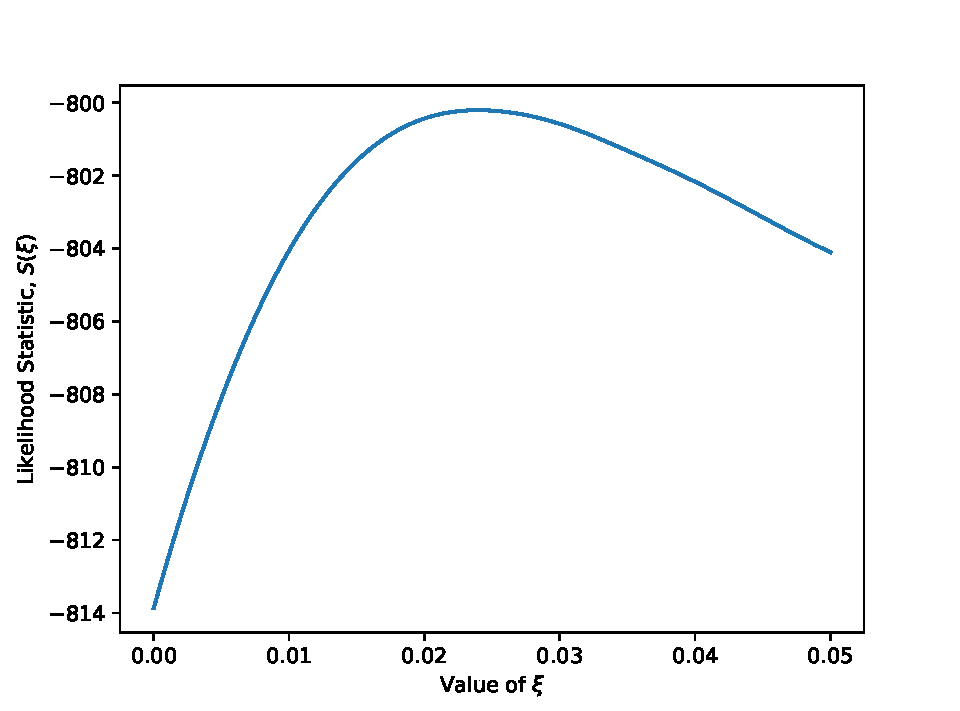
\includegraphics[width=1\textwidth]{{Figures/xi_plot.pdf}}
	\captionof{figure}{S($\xi$) vs $\xi$: The maximum occurs at $\xi = 0.024$.}
	\label{fig:play_by_play}
\end{figure}

\section{Dixon and Robinson}
Dixon and Robinson proposed an extension on the static Dixon and Coles model by incorporating the individual goal times.

\subsection{Model}
Dixon and Robinson began by 

It was clear that the Dixon and Coles model is more suitable for basketball and those team abilities will be used moving forward.
\section{Some Math Stuff}
The numbers can be seen in Table.  Using these numbers, and selecting the team with the highest probability of winning a game.  The accuracy of selecting a winner was 63.84\% and the value betting strategy won 57.84 units with 37.06\% winning bets.

Tried the Dixon and Coles model with a time parameter of 0.02 and the values seem more accurate.  The accuracy of selecting a winner was 63.21\% and the value betting strategy won 63.55 units with 38.03\% betting accuracy.  Did only the 2016 season and 64\% with the new vectorized way of doing it and 63.25 units.

Vectorized Dixon Coles and went from like 1341 seconds to 9 seconds for 3 seasons worth.  For some reason when I do Dixon Coles with the time factor with 2014, 2015 it gives me weird numbers but works perfectly fine with 2016 and 2017.  Must be something with the dataset
In the Dixon-Robinson model,.  By looking at NBA statistics the final minute of each quarter is likely to have an increase in scoring.


Dixon and Robinson model 1 is shown in Table \ref{table:dr_1_141516}.  The accuracy of selecting a winner was 60.28\% and the value betting strategy won 98.14 units with 37.31\% betting accuracy.

The issue with the betting is that it likes to bet on very high odds as the model computes probabilities differently.  Odds over 5 are usually bet.


\begin{equation}
    \lambda_k(t) = 
    \begin{cases}
        \rho_{1}\lambda_{xy}\lambda_{k} & \text{for }t \in (11/48, 12/48],\\
        \rho_{2}\lambda_{xy}\lambda_{k} & \text{for }t \in (23/48, 24/48],\\
        \rho_{3}\lambda_{xy}\lambda_{k} & \text{for }t \in (35/48, 36/48],\\
        \rho_{4}\lambda_{xy}\lambda_{k} & \text{for }t \in (47/48, 48/48],\\
        \lambda_{xy}\lambda_{k} & \text{otherwise}
\end{cases}
\end{equation}

The away rate is similar $\mu_k(t)$.



The optimal value is 0.024.

\section{Team Model}

Just like the model from Section a, with $n$ teams, the offence parameters $\{\alpha_1,\ldots,\alpha_n\}$ $\{\beta_1,\ldots,\beta_n\}$ $\gamma_h$ are to be estimated.  The following constraint is imposed due to the 

$$\frac{1}{n}\sum^{n}_{i=1}\alpha_i = 100$$

For the NBA, there are 30 teams, which gives a total of 61 parameters to be estimated.

\section{Player Model}

\chapter{Player Model}\label{chapter:player_model}


\chapter{Prediction Results}\label{chapter:prediction_results}
Probabilities for each team to win were generated using equation (\ref{eq:prob}).  Since the abilities for each week were obtained by data from the previous ones, predictions for all seasons can be done.  The model chooses the winner by selecting the team with the higher probability.

\chapter{Sports Betting}\label{chapter:betting}

Using the model developed in the previous section, we can take a look at the betting markets.  Betting odds used in betting markets are simply a probability of a team winning.  So we will use the probabilities generated from our model and compare them to the betting odds to determine where we should place our money.

\textit{Look at Pope and Peel (1989) and Dixon and Pope (1006)}

Using historical odds for the 2014-15, 2015-16 and 2016-17 seasons, we are able to determine the betting proficiency of the model.  We are using model (4.52), with $\xi = 0.062$ and $\omega=0.17$ at each time point to estimate the results.  Once probabilities for matches are obtained, we can compare with the bookies' odds to determine which match should be bet and calculating the profit.

\section{Betting Strategy}
In order to maximize profits, a number of betting strategies were implemented.

The parameters obtained to maximize the prediction accuracy might not accurately reflect the probabilities outputted by the model for the betting market.  Thus, to obtain new values of $\xi$ and $\omega$ the following equation will be used.

\begin{equation}\label{eq:score}
S(\xi) = \sum_{k=1}^{N}(\delta_k^H\log p_k^H + \delta_k^A \log p_k^A)
\end{equation}

where, $\delta_k^H = 1$ if match $k$ was a home win and $\delta_k^H=0$ otherwise and vice versa for $\delta_k^A$.  As shown in Figure 2, the function is maximised at $\xi = 0.102$.  Equation (\ref{eq:score}) is also used to maximise the value of $\omega$ as shown in Figure 3.  The value is maximised at $\omega = 33.2$.

\chapter{Fantasy Basketball}\label{chapter:fantasy}

\chapter{Conclusion}\label{chapter:conclusion}
In conclusion

To further improve the model, 

%% ----------------------------------------------------------------
% Now begin the Appendices, including them as separate files

\addtocontents{toc}{\vspace{2em}} % Add a gap in the Contents, for aesthetics

\appendix % Cue to tell LaTeX that the following 'chapters' are Appendices

\chapter{Basketball Reference}

\begin{figure}[h]
\centering
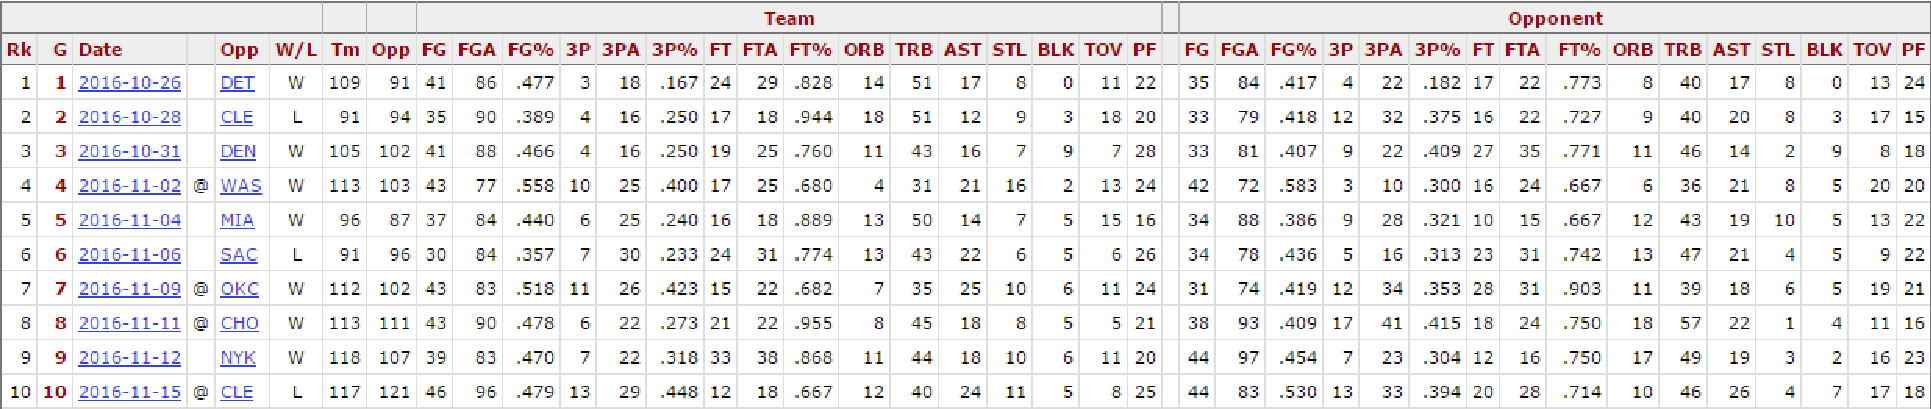
\includegraphics[width=1\textwidth]{{Figures/raptors_gamelog.pdf}}
\captionof{figure}{Game Logs of the Toronto Raptors in the 2016-2017 Regular Season \citep{basketball_reference}}
\label{fig:game_logs}
\end{figure}

\begin{figure}[h]
\centering
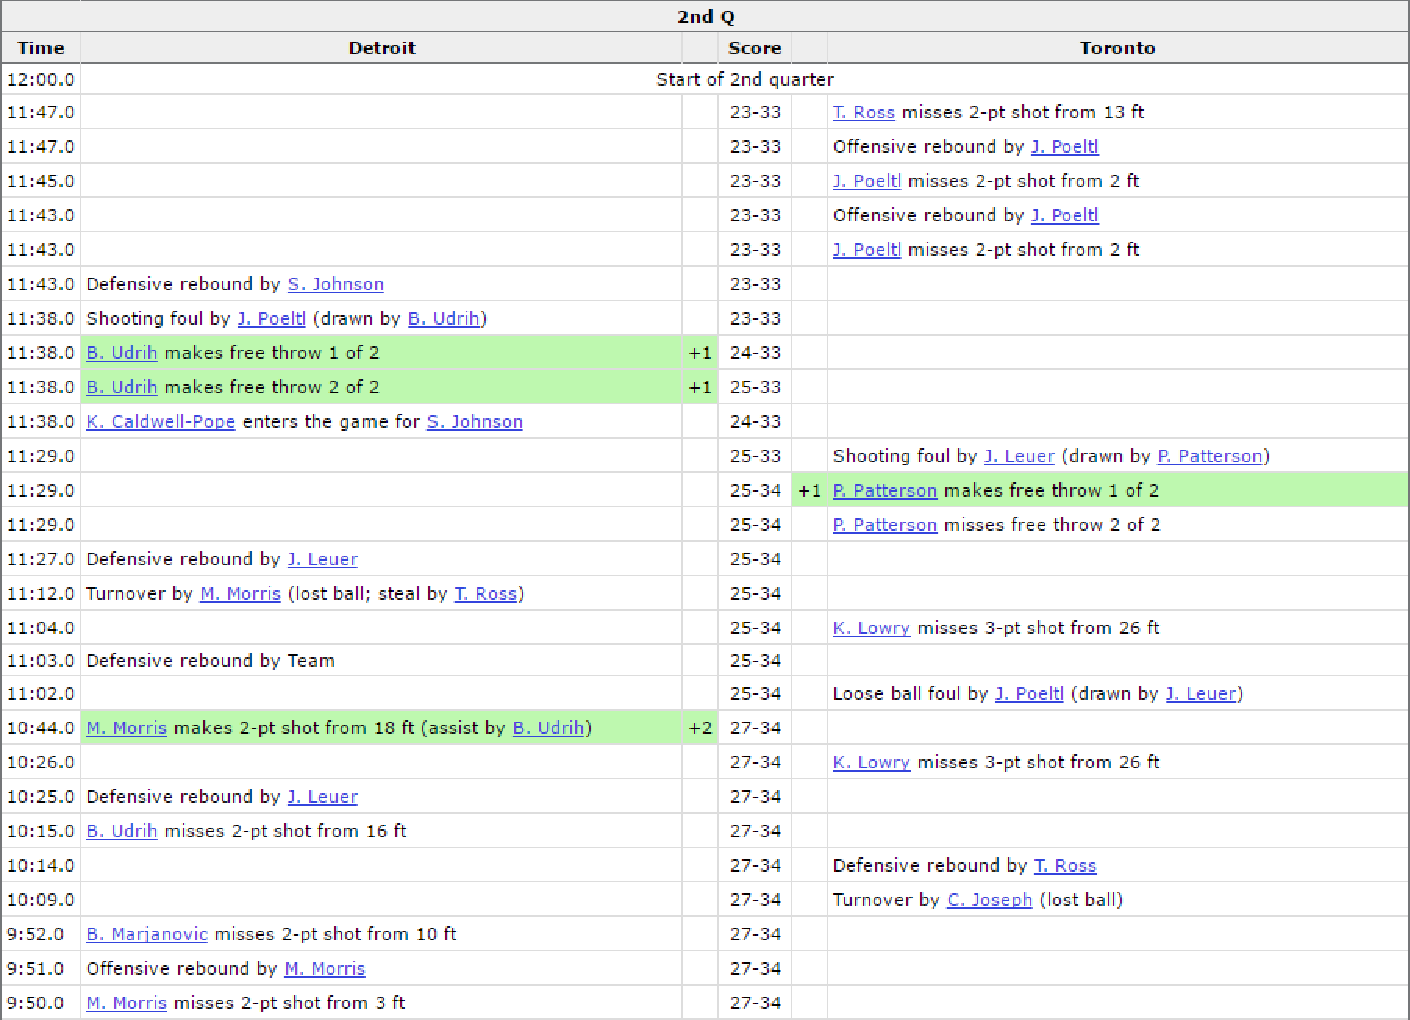
\includegraphics[width=1\textwidth]{{Figures/raptors_pbp.pdf}}
\captionof{figure}{Snippet of the play by play between Toronto and Detroit}
\label{fig:play_by_play}
\end{figure}
	% Appendix Title


%\input{Appendices/AppendixC} % Appendix Title

\addtocontents{toc}{\vspace{2em}}  % Add a gap in the Contents, for aesthetics
\backmatter

%% ----------------------------------------------------------------
\label{Bibliography}
\lhead{\emph{Bibliography}}  % Change the left side page header to "Bibliography"
\bibliographystyle{unsrtnat}  % Use the "unsrtnat" BibTeX style for formatting the Bibliography
\bibliography{Bibliography}  % The references (bibliography) information are stored in the file named "Bibliography.bib"

\end{document}  % The End
%% ----------------------------------------------------------------